\documentclass{myBeamer}

%% Title page
\title{Ordinary Differential Equations}
\subtitle{as an alternative to agent-based modelling}
\author{eX Modelo school}
\date{June 26, 2019}
\institute{
\includegraphics[scale=1.5]{figures/logos/openmole.png}}


\begin{document}

\begin{frame}[plain]
	\titlepage
\end{frame}
\addtocounter{framenumber}{-1}

\AtBeginSection[]
{
	\frame{
		\sectionpage
	}
	\addtocounter{framenumber}{-1}
}


\section{ODE systems}

\sframe{The ODE framework}{
	$\rightarrow$ widely used to model transmission phenomena\\
	
	\bigskip
	
	\begin{columns}
	\begin{column}{.5\textwidth}
		\begin{itemize}
			\item population split into compartments
			\item system of ordinary differential equations
		\end{itemize}
	\end{column}
	
	\begin{column}{.5\textwidth}
		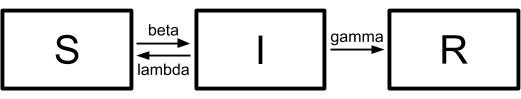
\includegraphics[width=\textwidth]{figures/SIR.jpg}\\
		
		\begin{eqnarray*}
		\left\{
		\begin{array}{lcl}
			\dv{S}{t}  & = &  -\beta S + \lambda I \\
			\tmspace{1mu}&& \\
			\dv{I}{t} & = & \beta S - (\lambda + \gamma)I \\
			\tmspace{1mu}&& \\
			\dv{R}{t} & = & \gamma I
		\end{array}
		\right.
		\end{eqnarray*}
	\end{column}
	\end{columns}
}


\sframe{SIR model dynamics}{
	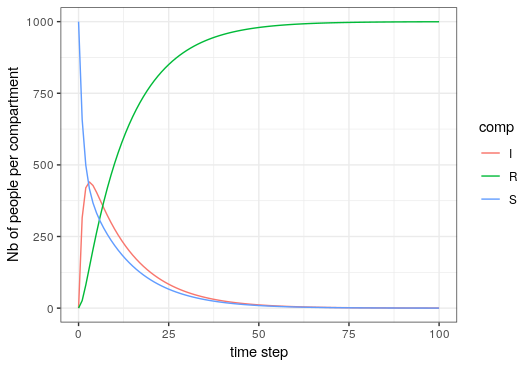
\includegraphics[width=\textwidth]{figures/SIR_dynamics.png}
}


\sframe{ODE vs ABM}{
	\begin{table}
 	\begin{tabular}{ll}
 		\thead{\head{ODE}} & \thead{\head{ABM}} \\
		Equation-based & Individual-based \\
		Generic mechanisms & Precise mechanisms \\
		Population scale & Individual scale \\
		Needs less resources & Computationally  expensive
  	\end{tabular}
  	\end{table}
}


\section{A Zombie situation}

\sframe{An ODE model for our Zombie problem}{
	\head{How could we model the Zombie invasion?}
	
	\begin{itemize}
		\item Which mechanisms?
		\item Which parameters?
	\end{itemize}
	
	\bigskip
	
	\visible<2>{
	\head{How can we assess our model's ability to reproduce the real data?}
	
	\begin{itemize}
		\item Which metrics?
		\item Which fitness function?
	\end{itemize}
	}
}


\sframe{A very simple ODE model}{
	\begin{center}
	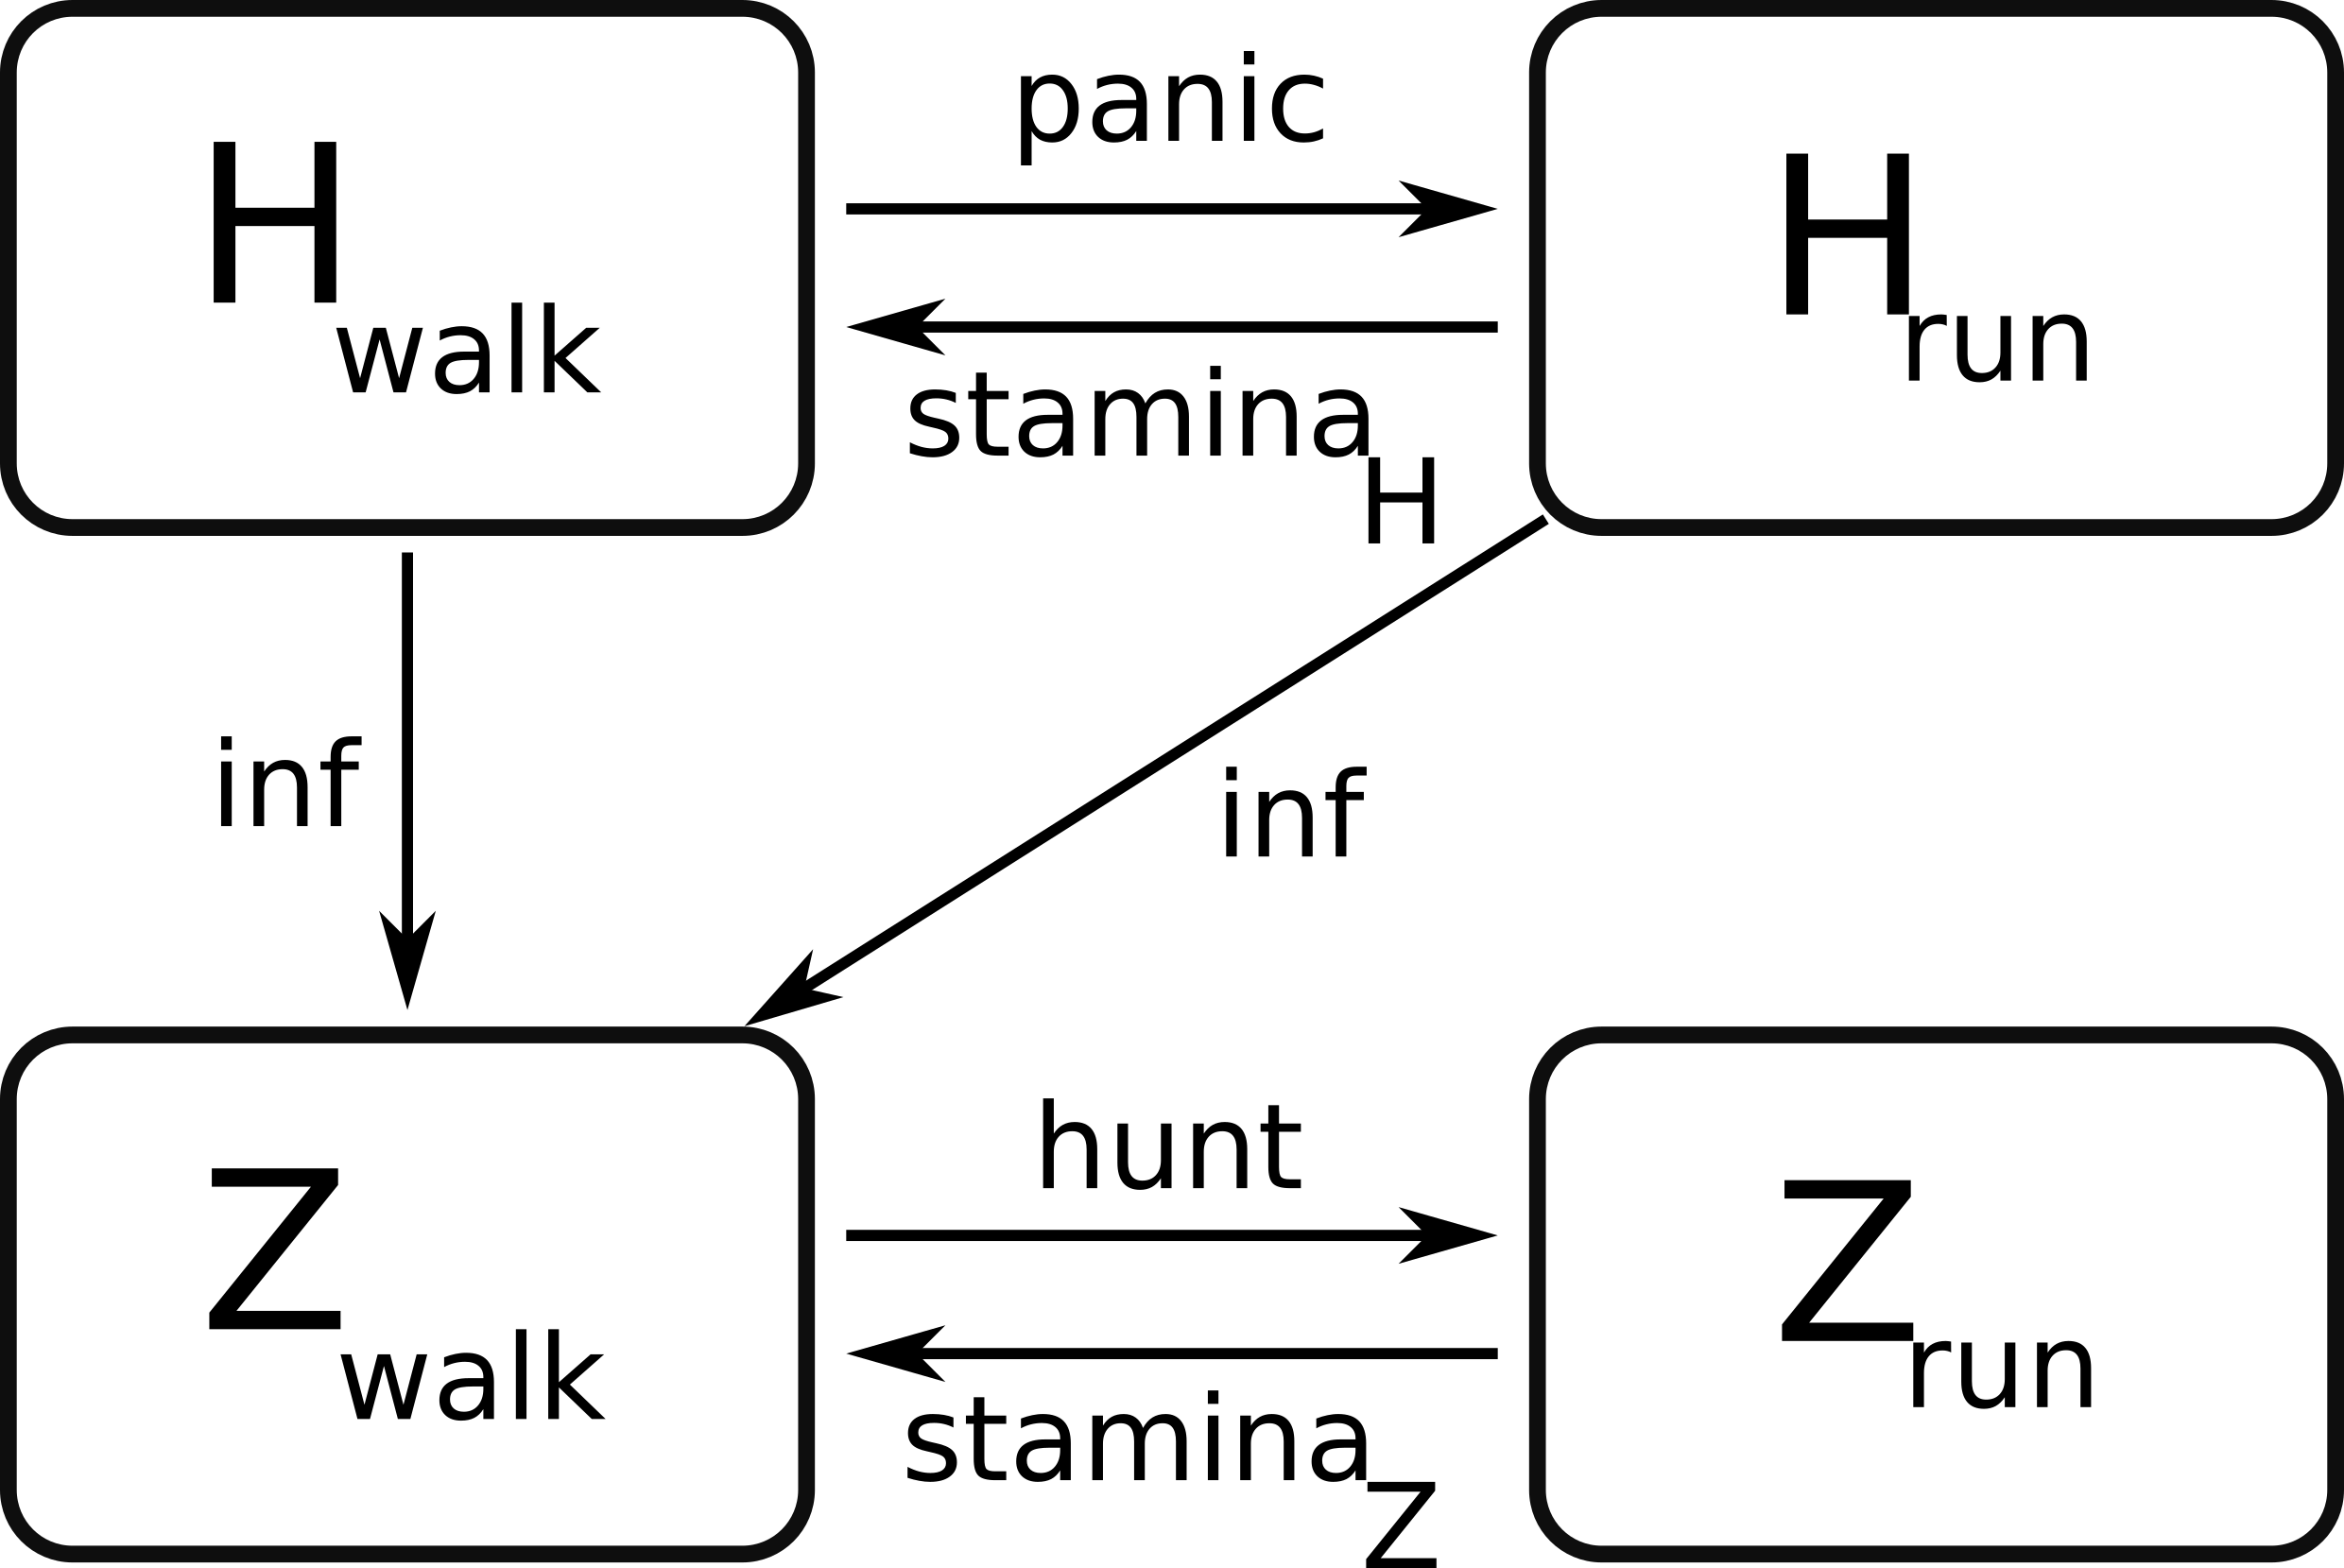
\includegraphics[width=.7\textwidth]{figures/simpleODE.png}
	\end{center}
}


\sframe{A very simple ODE model}{
	\begin{center}
	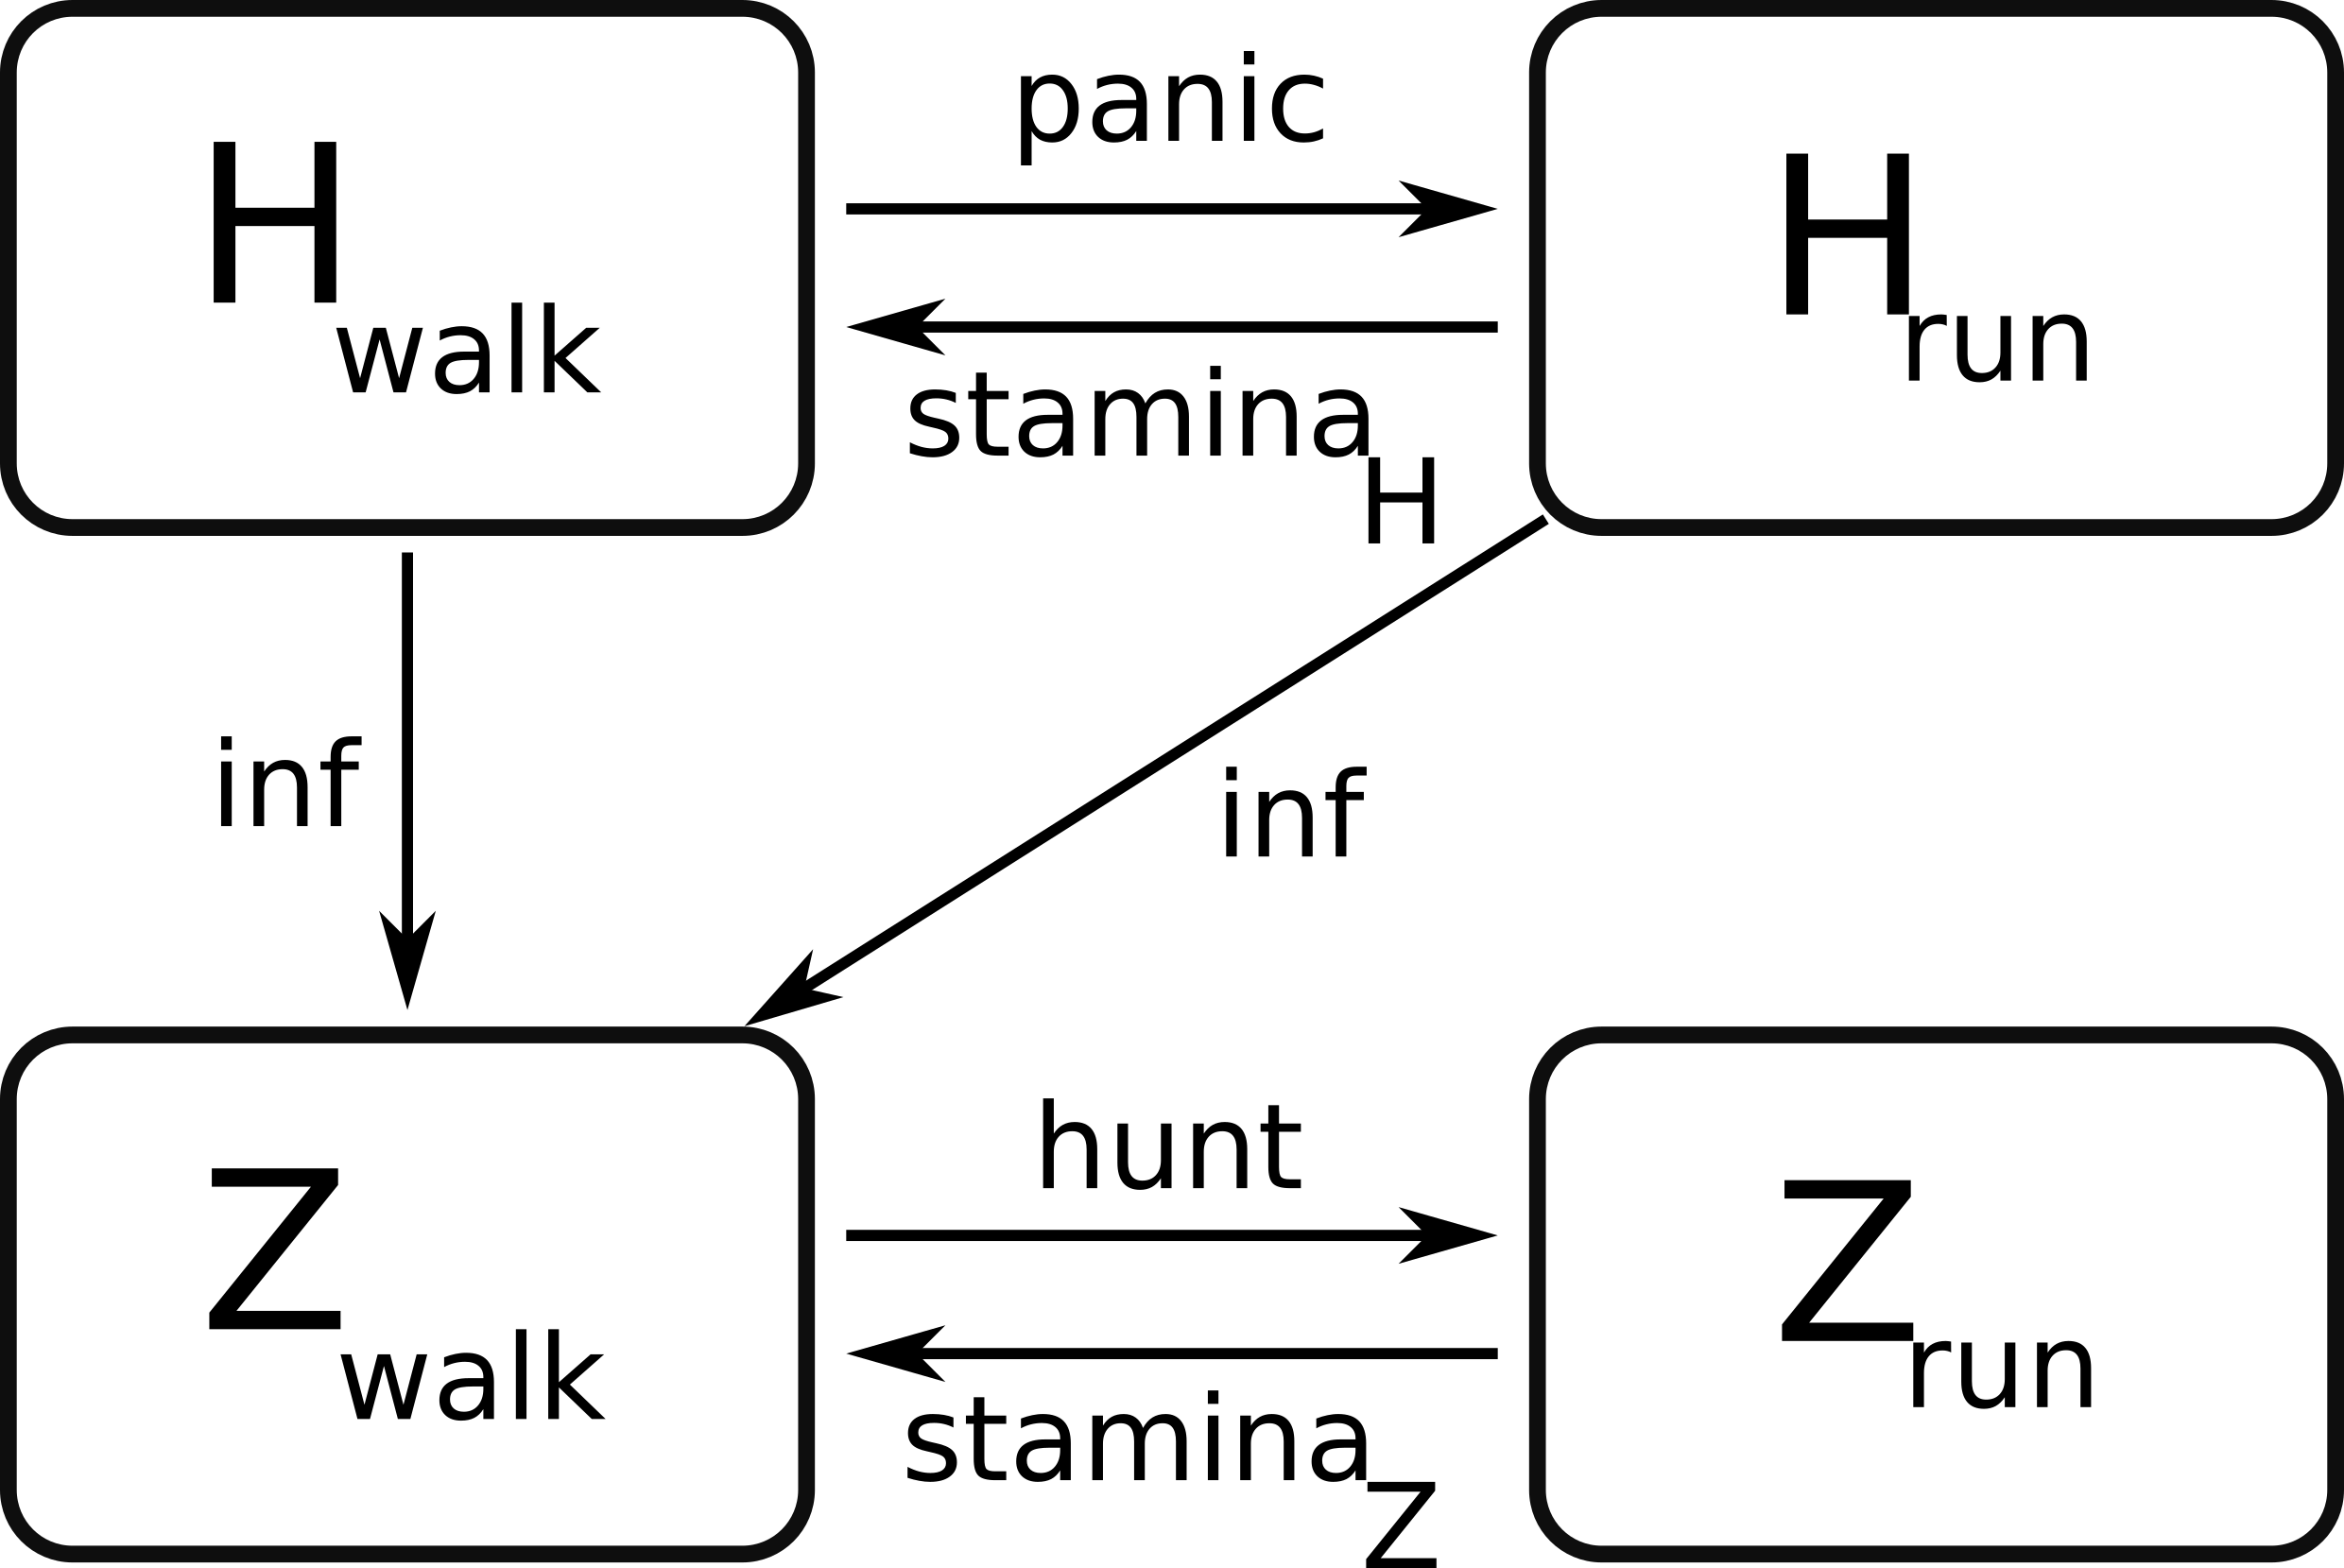
\includegraphics[width=.35\textwidth]{figures/simpleODE.png}
	\end{center}
	
	\begin{eqnarray*}
		\left\{
		\begin{array}{lcl}
			\dv{H_{walk}}{t}  & = &  -(panic + inf) * H_{walk} + exhaustH * H_{run} \\
			\tmspace{1mu}&& \\
			\dv{H_{run}}{t} & = & panic * H_{walk} - (exhaustH + inf) * H_{run} \\
			\tmspace{1mu}&& \\
			\dv{Z_{walk}}{t} & = & inf * (H_{walk} + H_{run}) - hunt * Z_{walk} + exhaustZ * Z_{run} \\
			\tmspace{1mu}&& \\
			\dv{Z_{run}}{t} & = & hunt * Z_{walk} - exhaustZ * Z_{run}
		\end{array}
		\right.
	\end{eqnarray*}
}


\section{Exploration}

\sframe{First step: Calibrate}{
	\begin{center}
	We have some real time series of zombie invasion \\
	$\rightarrow$ find the parameter values to best fit them
	\end{center}
	
	\bigskip
	
	\visible<2->{
	\head{Process}
	
	\begin{itemize}
		\visible<3->{\item Embed the model in OpenMOLE}
		\visible<4->{\item Define a fitness function}
		\visible<5->{\item Write a calibration task}
	\end{itemize}
	}
}


\sframe{Calibration results}{
	\head{Parameter set} \\
	
	\bigskip
	
%	\includegraphics[width=\textwidth]{figures/calib.png}
}


\sframe{Second step: Profiles}{

}


\section{Adding complexity}

\sframe{New mechanisms}{
	\begin{center}
	What mechanisms could we add to better represent the complexity of our Zombie situation?
	\end{center}
	
	\bigskip
	
	\visible<2->{
	\head{The parcimony issue}
	
	\begin{itemize}
		\visible<3->{\item Do the new mechanisms really improve the fitness?}
		\visible<4->{\item Do we need them all?}
		\visible<5->{\item What are the best combinations?}
	\end{itemize}
	}
}


\sframe{Study our model's parcimony}{
	\head{Process}
	
	\begin{itemize}[<+->]
		\item Embed the model in OpenMOLE \head{DONE}
		\item Define a \head{second} fitness function
		\item \head{Modify} the calibration task
	\end{itemize}
}


\sframe{Pareto front}{
	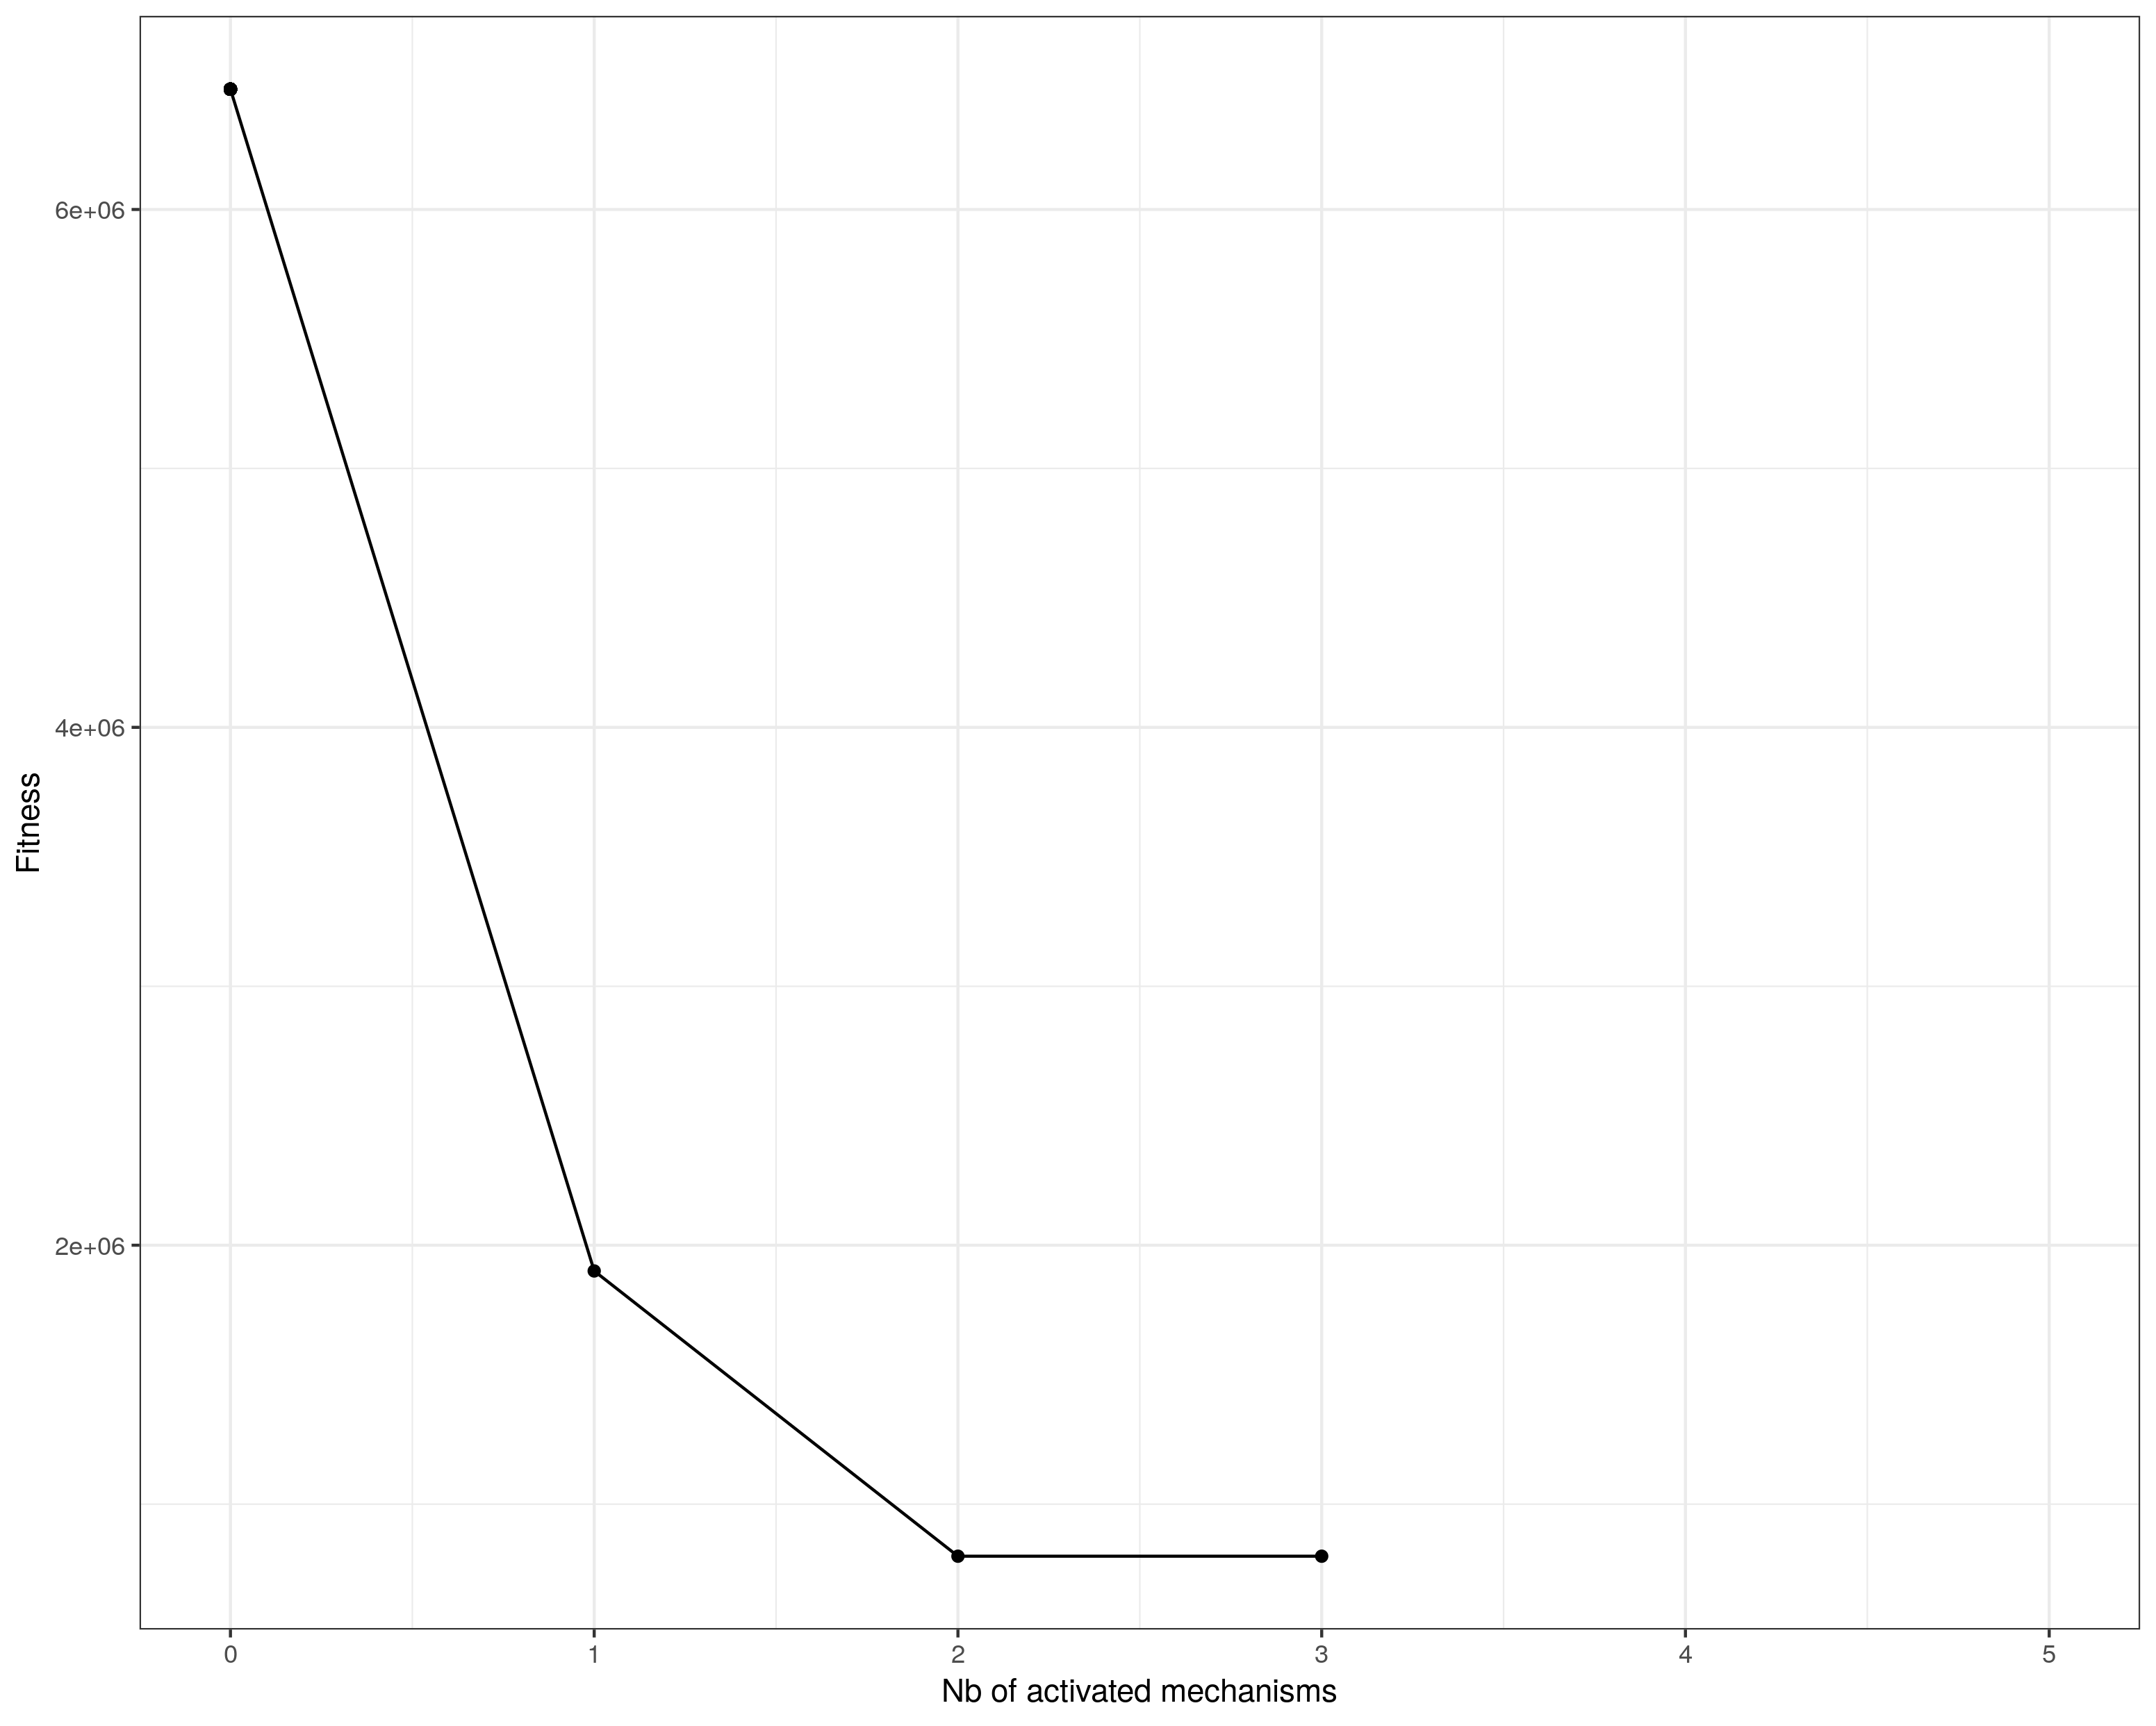
\includegraphics[width=\textwidth]{figures/parcimony/plot_parcimony.png}
}


\sframe{Dynamics for 0 mechanism activated}{
	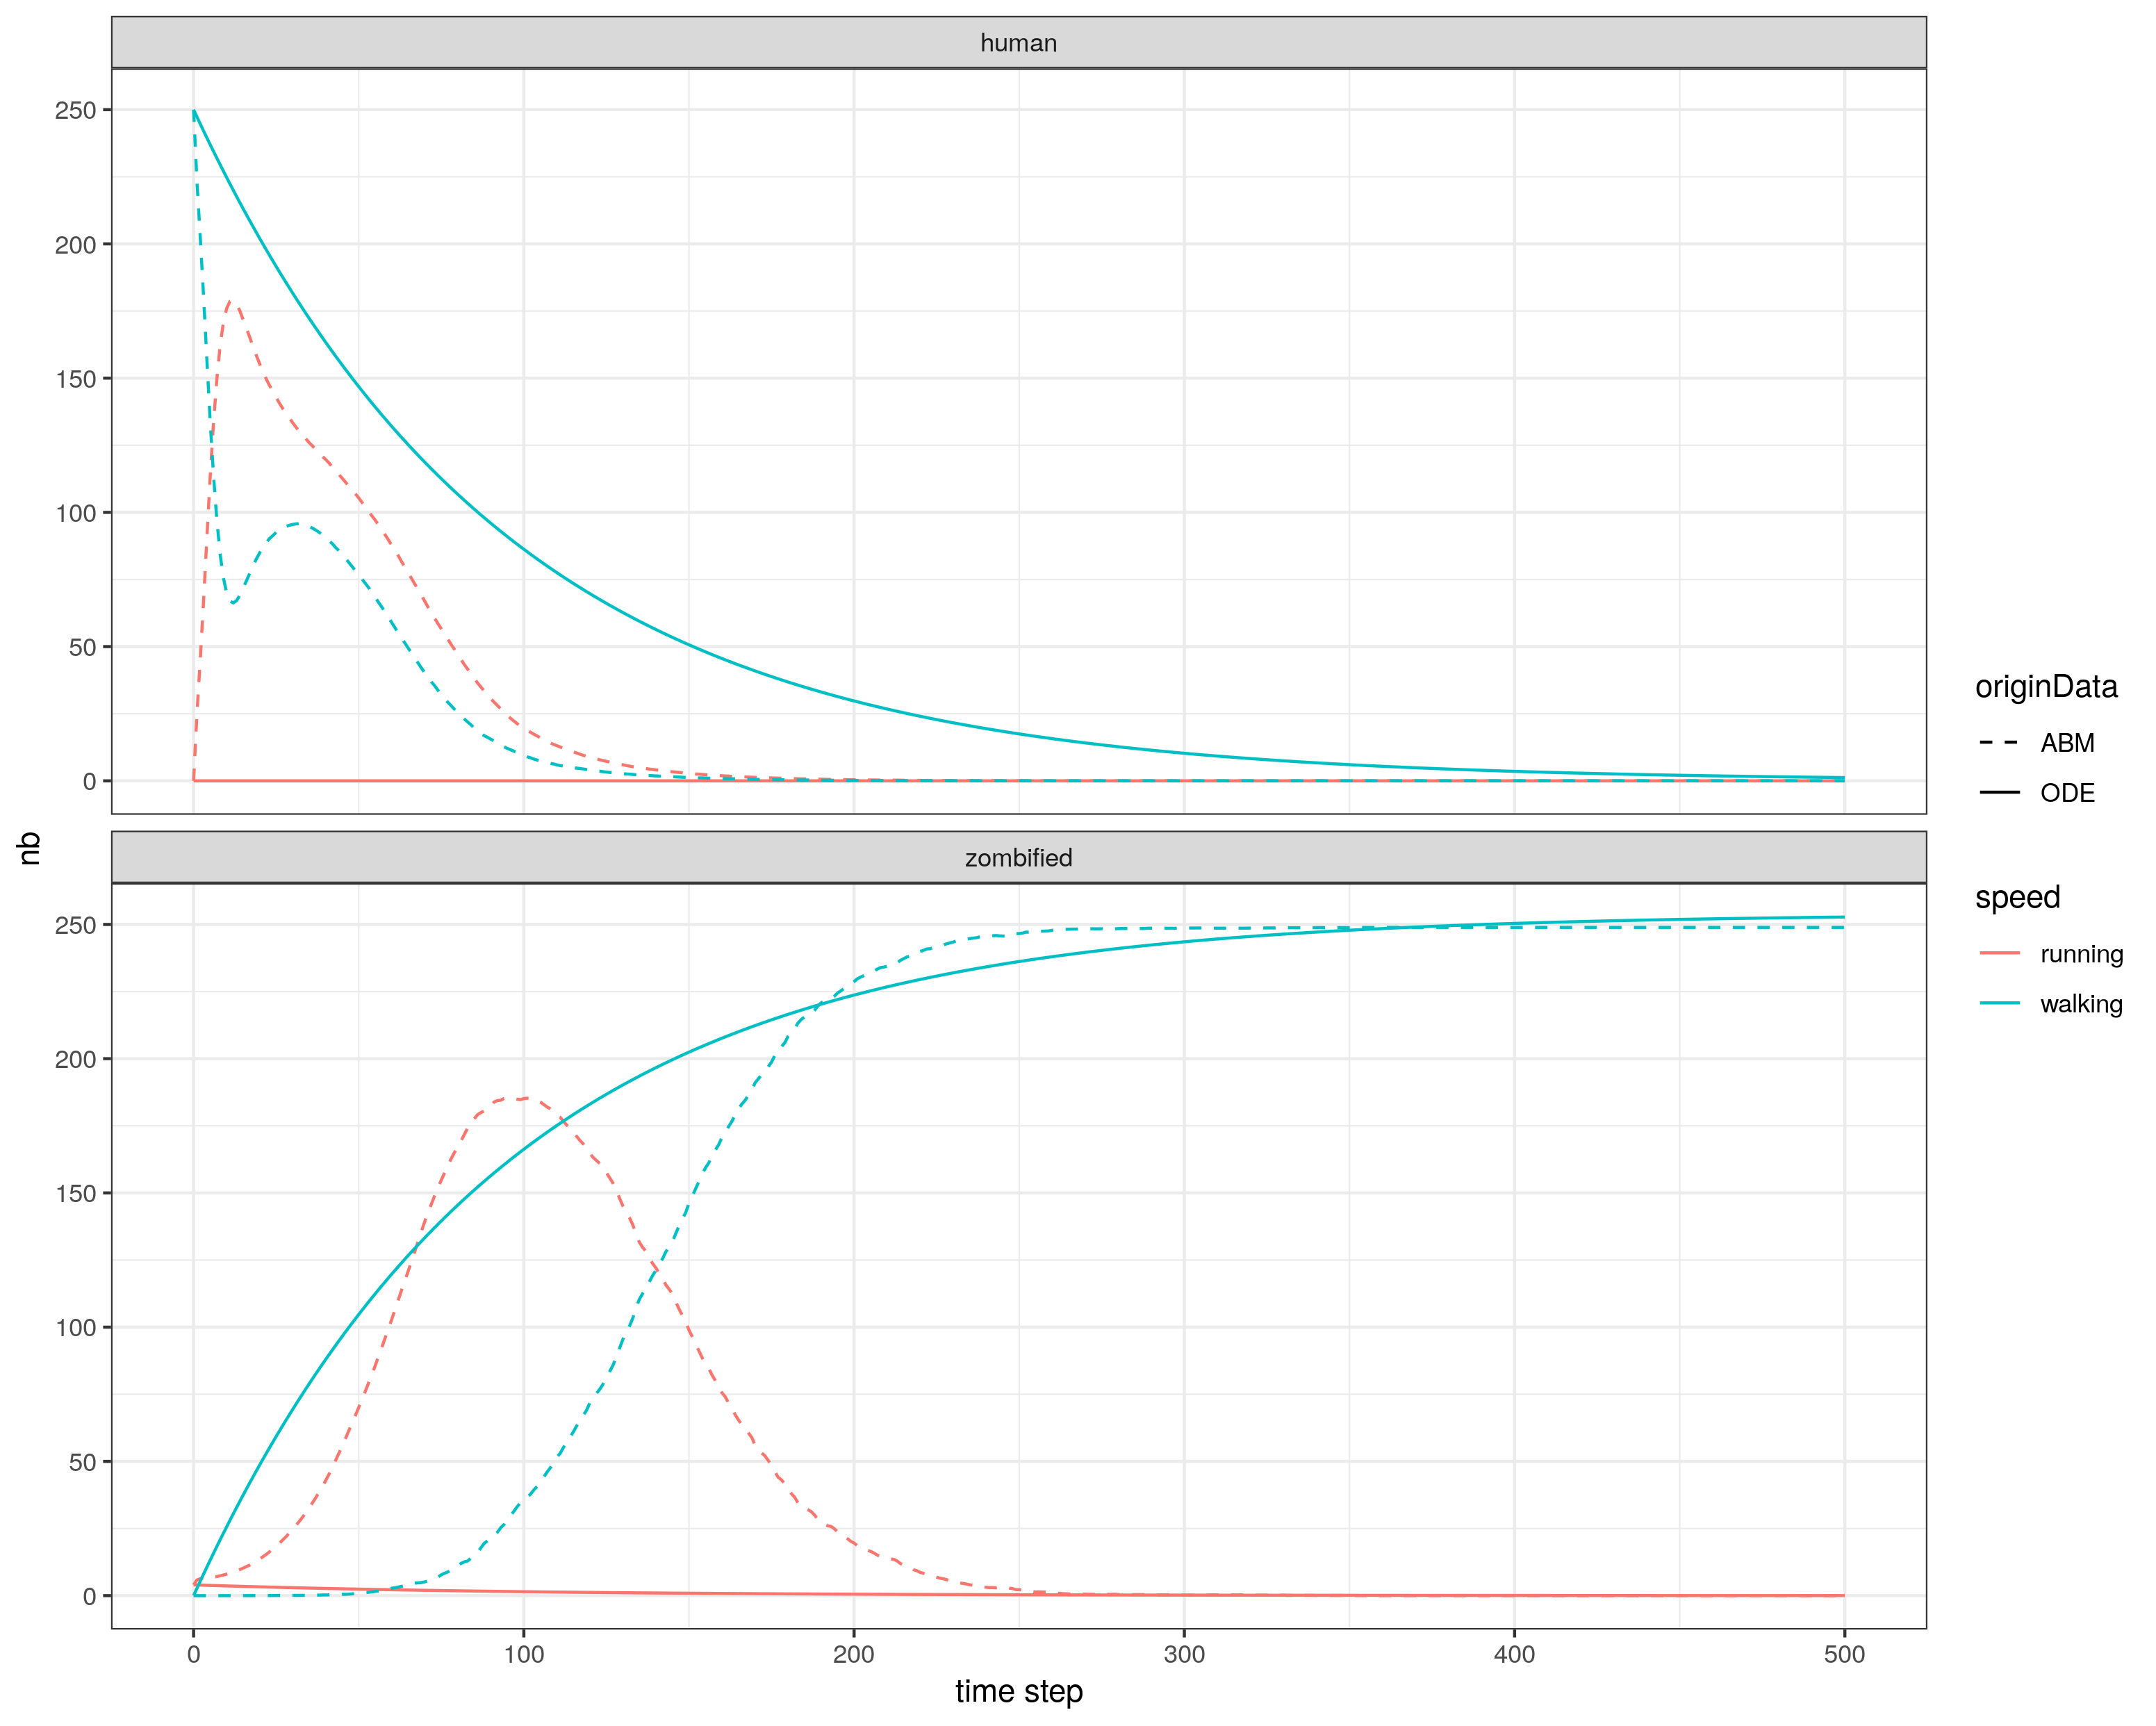
\includegraphics[width=\textwidth]{figures/parcimony/parcimony_dynamics_0.png}
}


\sframe{Dynamics for 1 mechanism activated}{
	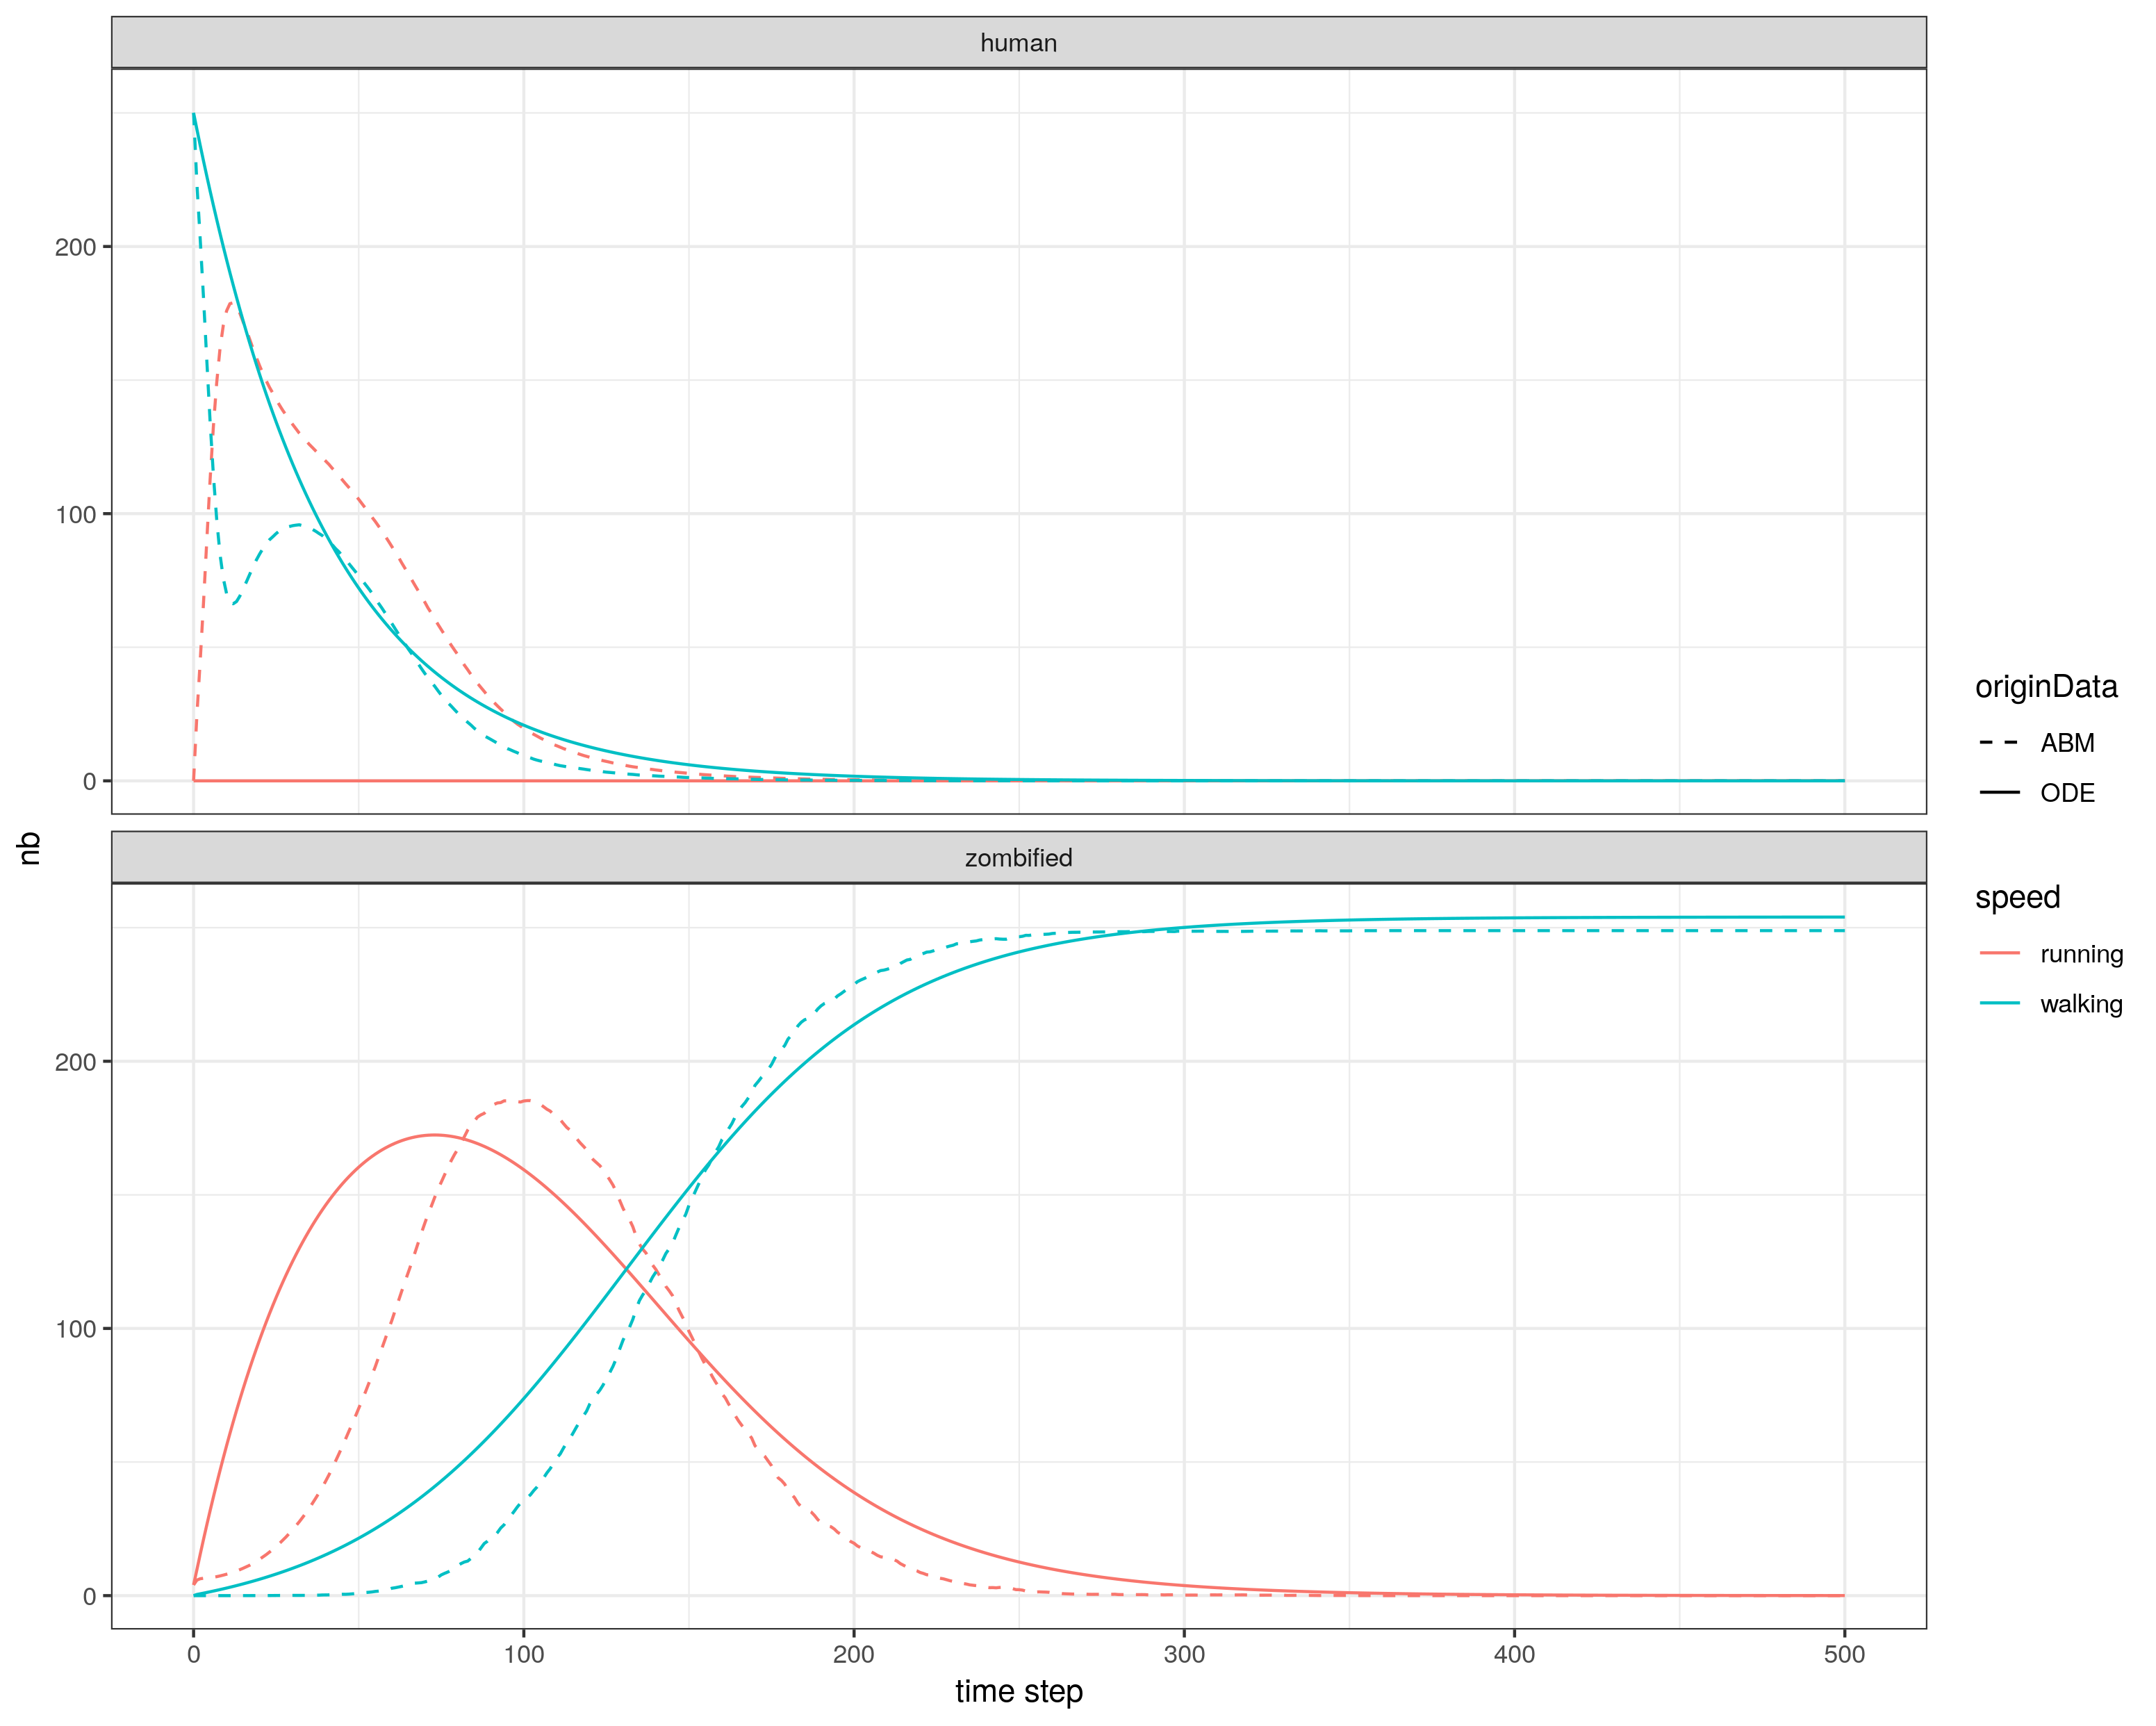
\includegraphics[width=\textwidth]{figures/parcimony/parcimony_dynamics_1.png}
}


\sframe{Dynamics for 2 mechanisms activated}{
	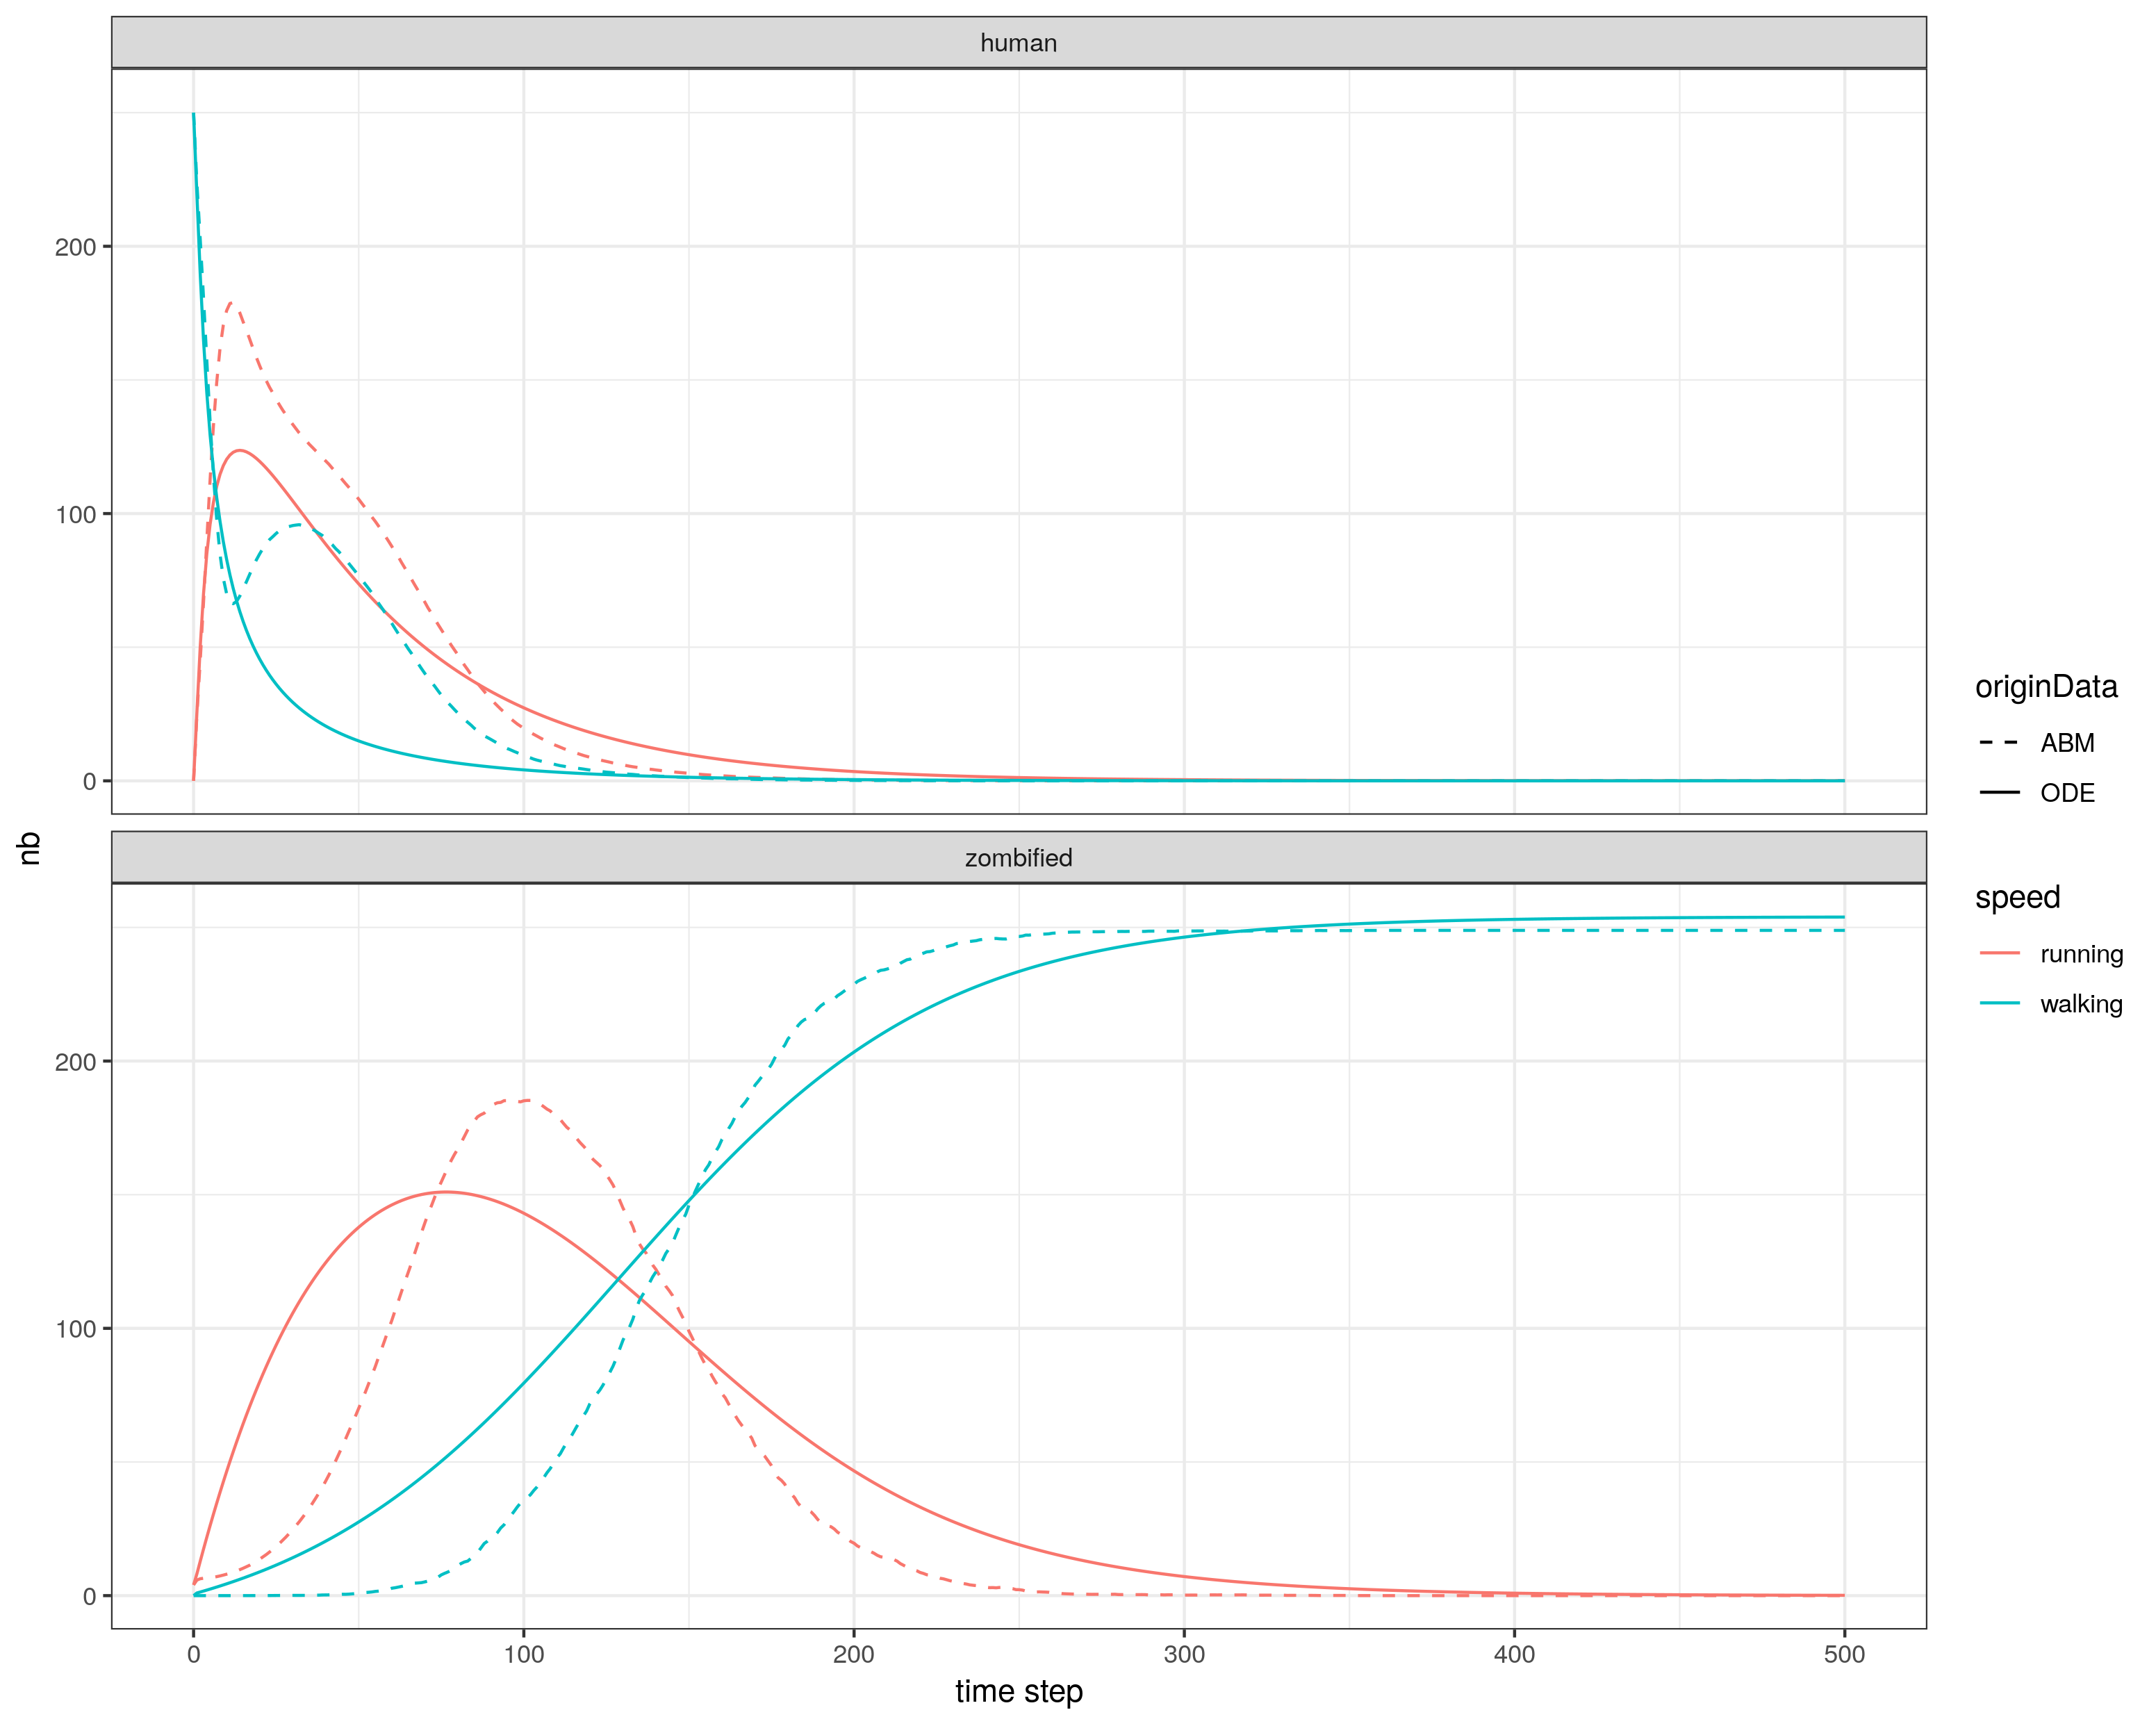
\includegraphics[width=\textwidth]{figures/parcimony/parcimony_dynamics_2.png}
}


\sframe{Dynamics for 3 mechanisms activated}{
	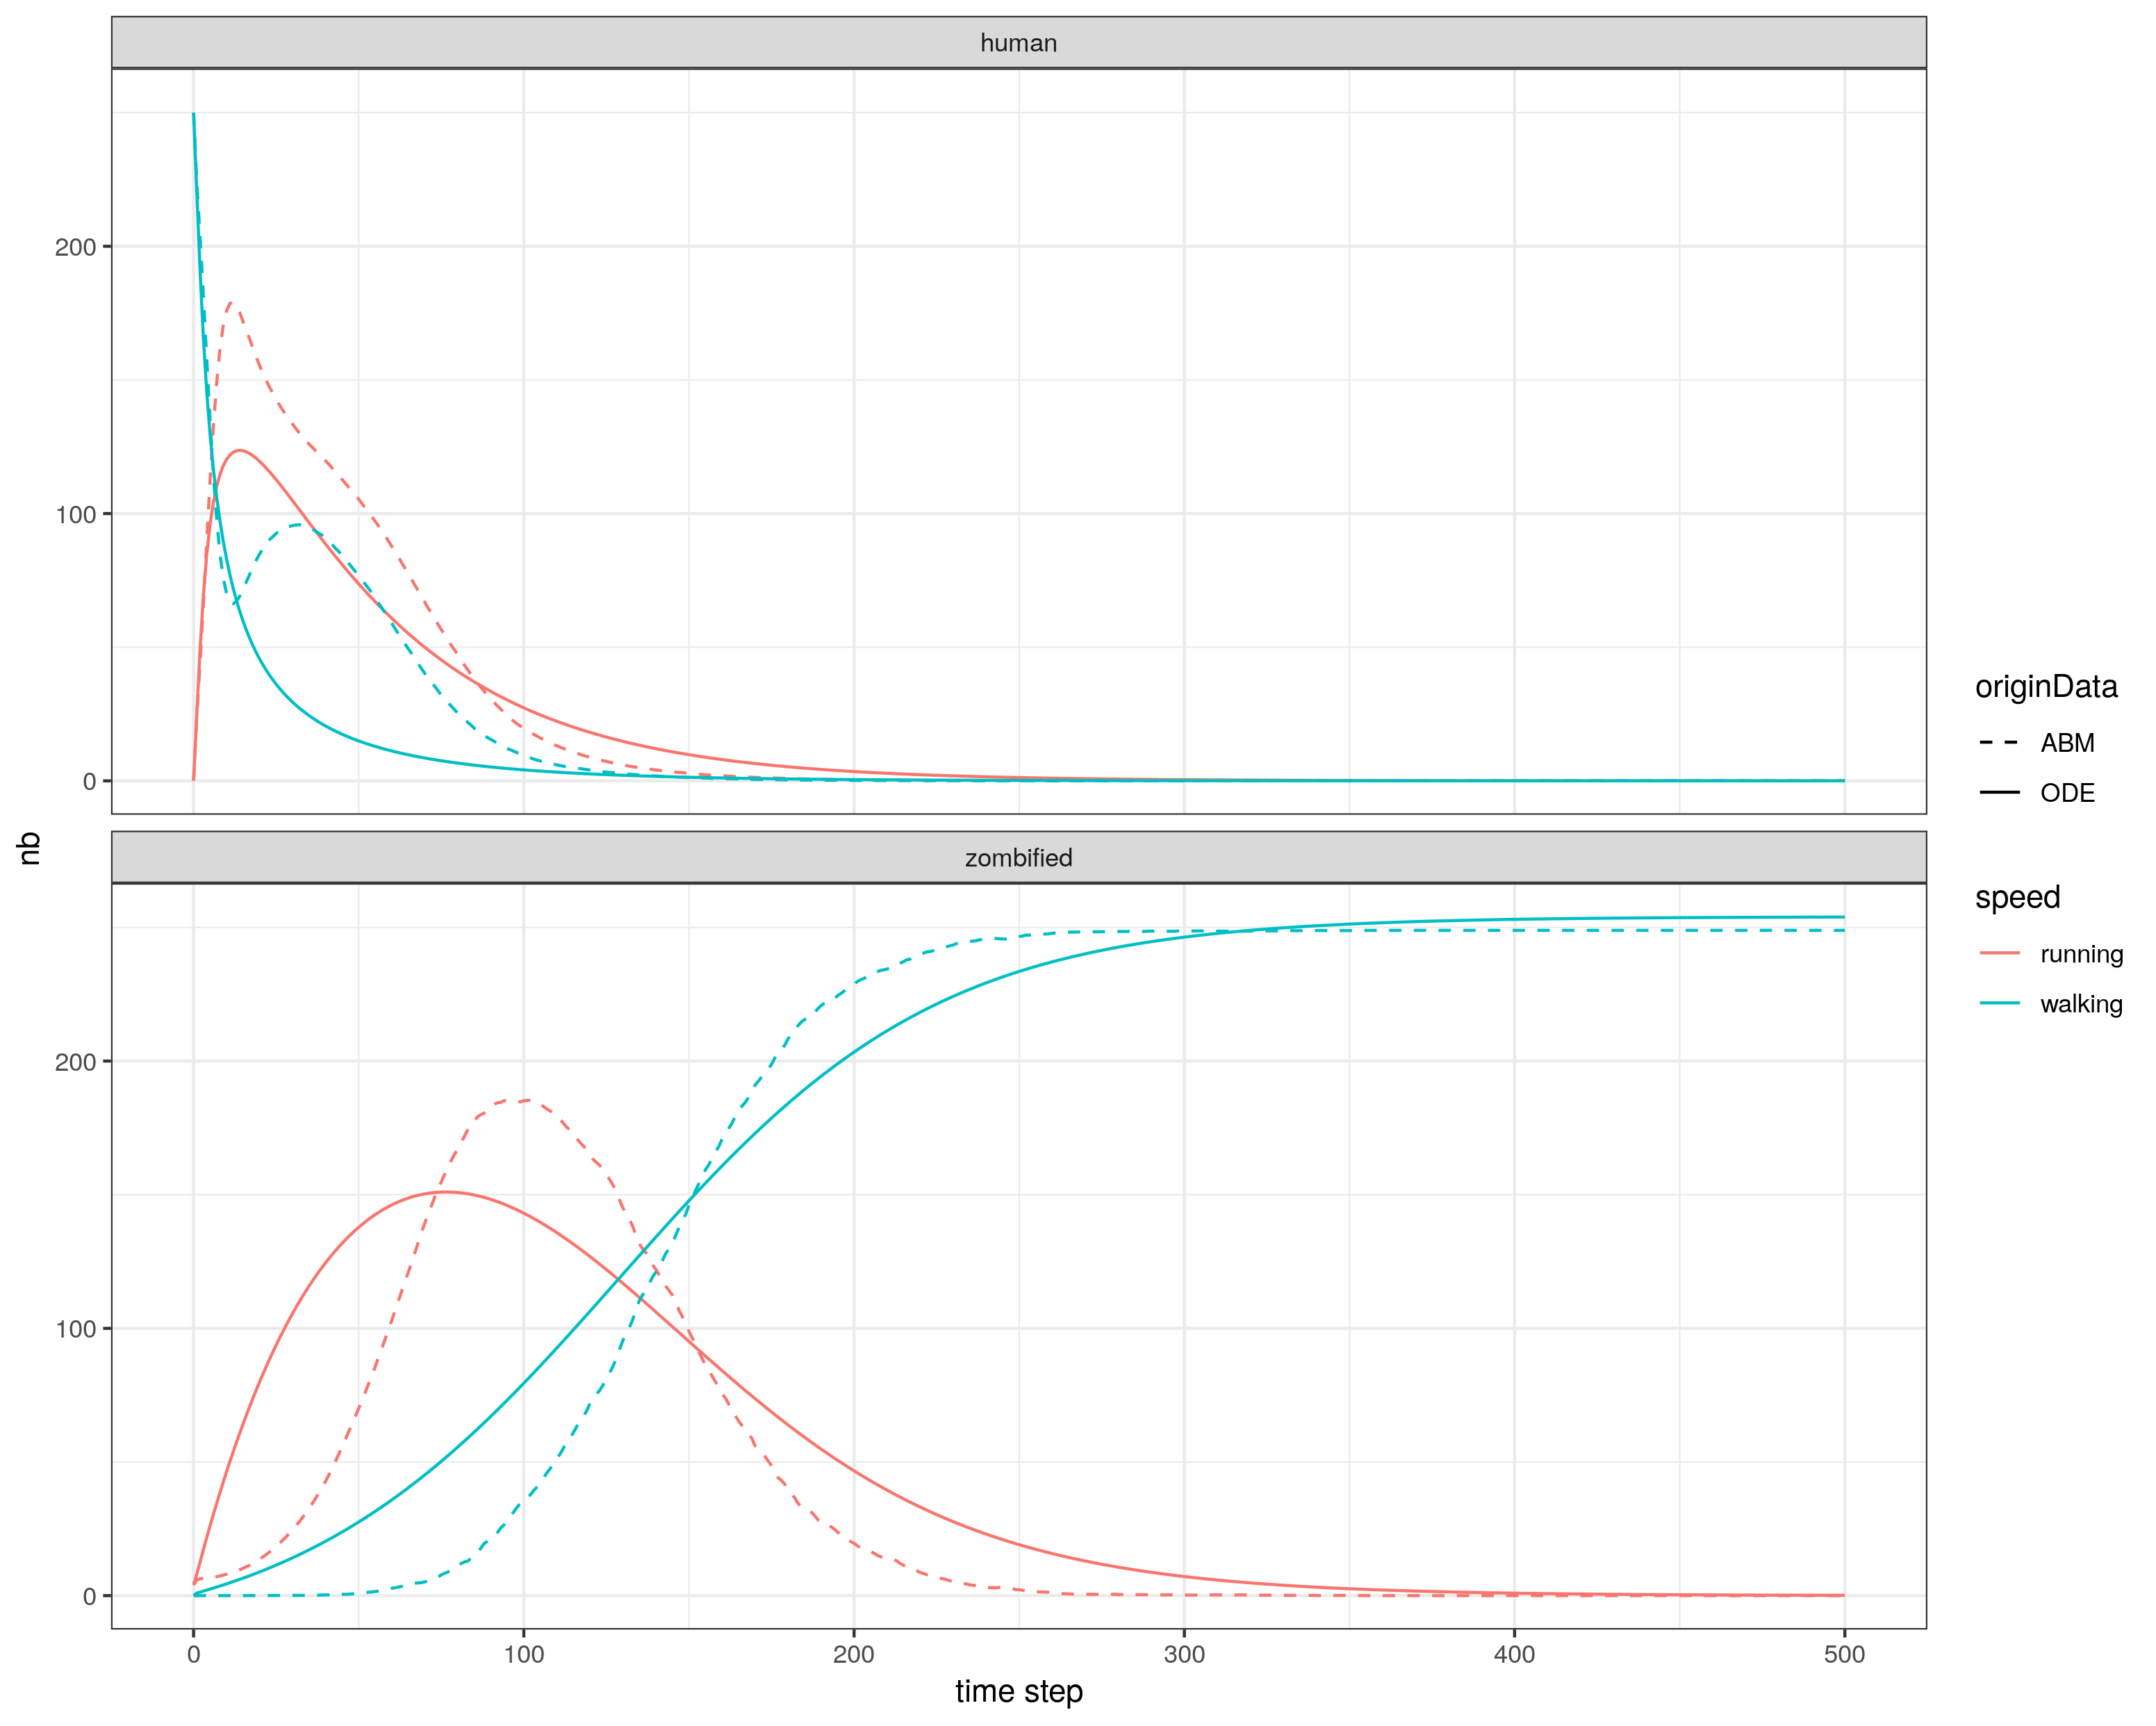
\includegraphics[width=\textwidth]{figures/parcimony/parcimony_dynamics_3.png}
}


%% Stop numbering
\backupbegin

\appendix
%\begin{frame}[plain]{Acknowledgements}
%	\begin{center}
%	\head{Lab:}\\
%	
%	\medskip
%	XXX\\
%	\medskip
%	YYY\\
%	\medskip
%	ZZZ\\
%	
%	\bigskip
%	Logos
%	\end{center}
%	
%	\visible<2>{
%	\bigskip
%	\begin{LARGE}
%		\begin{center}
%		\head{Thank you for your attention!}
%		\end{center}
%	\end{LARGE}
%	}
%\end{frame}

%\section{Annexes}
\subsection{Modèle SimFI}

%\begin{frame}[plain]
%	\begin{center}
%	{\LARGE \color{myDarkBlue}\bfseries Backup}
%	\end{center}
%\end{frame}


\begin{frame}{Déroulement d'un pas de temps}
	\begin{center}
	\includegraphics[width=.6\textwidth]{figures/backup/jour_type.png}
	\end{center}
\end{frame}


\begin{frame}{Modification des probabiblités de transmission}
	\begin{center}
	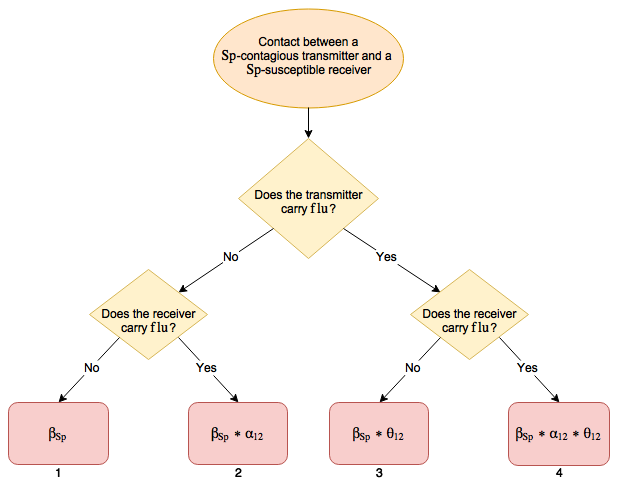
\includegraphics[width=.9\textwidth]{figures/backup/proba_interactions.png}
	\end{center}
\end{frame}


\begin{frame}{Excès de cas direct et indirect}
	\begin{center}
	\includegraphics[width=\textwidth]{figures/backup/Figure_4.png}
	\end{center}
\end{frame}


\begin{frame}{Morbidité de la grippe liée à l'interaction}
	\begin{center}
	\includegraphics[width=.8\textwidth]{figures/backup/burdenFlu.png}
	\end{center}
\end{frame}


\begin{frame}{Résultats des régressions linéaires}{Scénarios avec saison intrinsèque}
\vspace{-.4cm}
	\begin{center}
	\includegraphics[width=.95\textwidth]{figures/backup/Lineaire_moyplot_cosSeason.png}
	\end{center}
\end{frame}


\begin{frame}{Résultats des régressions linéaires}{Scénarios sans saison intrinsèque}
\vspace{-.4cm}
	\begin{center}
	\includegraphics[width=.95\textwidth]{figures/backup/Lineaire_moyplot_noSeason.png}
	\end{center}
\end{frame}


\begin{frame}{Résultats des régressions binomiales négatives}{Scénarios avec saison intrinsèque}
\vspace{-.4cm}
	\begin{center}
	\includegraphics[width=.95\textwidth]{figures/backup/NegBin_moyplot_cosSeason.png}
	\end{center}
\end{frame}


\begin{frame}{Résultats des régressions binomiales négatives}{Scénarios sans saison intrinsèque}
\vspace{-.4cm}
	\begin{center}
	\includegraphics[width=.95\textwidth]{figures/backup/NegBin_moyplot_noSeason.png}
	\end{center}
\end{frame}


\begin{frame}{Estimation des paramètres d'interaction}{Scénarios avec saison intrinsèque}
\vspace{-.3cm}
\begin{table}
	\begin{center}
	\makegapedcells
	\begin{tiny}
	\begin{tabular}{|c|c|rl|rl|}
		\hline
		\thead{Excès\\d'infections\\à pneumocoque} & \thead{Force\\d'interaction\\correspondante} & \thead{$\xi$} & \thead{IC 95\%} & \thead{$\pi$} & \thead{IC 95\%} \\
		\hline
		\multicolumn{6}{|c|}{\thead{Scénario de référence}} \\
		\hline
		0\% & $A=\Theta=\Pi=1$ & -0,001 & [-0,001 ; 4,545] & {\color{red}100,830} & {\color{red}[81,944 ; 130,066]} \\
		\hline
		\multicolumn{6}{|c|}{\thead{Mécanisme sur l'acquisition}} \\
		\hline
		2\% & $A=2$ & -0,001 & [-0,001 ; 13,514] & {\color{red}78,581} & {\color{red}[54,983 ; 98,001]} \\
		\hline
		5\% & $A=4$ & -0,001 & [-0,001 ; 9,000] & {\color{red}121,619} & {\color{red}[97,783 ; 146,023]} \\
		\hline
		10\% & $A=10$ & {\color{red}16,355} & {\color{red}[2,481 ; 31,022]} & {\color{red}164,999} & {\color{red}[130,986 ; 203,863]} \\
		\hline
		15\% & $A=50$ & {\color{red}31,987} & {\color{red}[17,467 ; 49,005]} & {\color{red}162,158} & {\color{red}[126,795 ; 199,617]} \\
		\hline
		\multicolumn{6}{|c|}{\thead{Mécanisme sur la transmission}} \\
		\hline
		2\% & $\Theta=2$ & -0,001 & [-0,001 ; 6,007] & {\color{red}82,425} & {\color{red}[65,134 ; 100,587]} \\
		\hline
		5\% & $\Theta=3$ & {\color{red}0,036} & {\color{red}[0,036 ; 7,536]} & {\color{red}92,008} & {\color{red}[67,739 ; 117,020]} \\
		\hline
		10\% & $\Theta=7$ & {\color{red}25,631} & {\color{red}[11,956 ; 40,504]} & {\color{red}142,500} & {\color{red}[112,488 ; 177,552]} \\
		\hline
		15\% & $\Theta=10$ & {\color{red}35,258} & {\color{red}[20,992 ; 51,001]} & {\color{red}143,008} & {\color{red}[113,975 ; 177,124]} \\
		\hline
		20\% & $\Theta=15$ & {\color{red}31,047} & {\color{red}[15,950 ; 47,023]} & {\color{red}202,876} & {\color{red}[166,739 ; 247,408]} \\
		\hline
		\multicolumn{6}{|c|}{\thead{Mécanisme sur la pathogénicité}} \\
		\hline
		2\% & $\Pi=5$ & -0,001 & [-0,001 ; 5,504] & {\color{red}111,008} & {\color{red}[89,259 ; 133,520]} \\
		\hline
		5\% & $\Pi=10$ & -0,001 & [-0,001 ; 2,533] & {\color{red}158,329} & {\color{red}[132,847 ; 186,098]} \\
		\hline
		10\% & $\Pi=20$ & -0,001 & [-0,001 ; 2,019] & {\color{red}219,443} & {\color{red}[192,420 ; 249,370]} \\
		\hline
		15\% & $\Pi=28$ & -0,001 & [-0,001 ; 2,023] & {\color{red}277,766} & {\color{red}[245,166 ; 311,543]} \\
		\hline
		20\% & $\Pi=40$ & -0,001 & [-0,001 ; 1,641] & {\color{red}365,054} & {\color{red}[325,374 ; 400,138]} \\
		\hline
	\end{tabular}
	\end{tiny}
	\end{center}
\end{table}
\end{frame}


\begin{frame}{Algorithme NSGA-2}
		\begin{enumerate}
			\item Initialisation d'un ensemble de jeux de paramètres $\{\theta_1,...,\theta_N\}$ de manière aléatoire
			\item Calcul de la vraisemblance pour chacun des $\theta_i$, $i \in \{1,N\}$
			\item Sélection de $K$ jeux de paramètres selon leur vraisemblance, par une méthode de tri rapide non dominé
			\item Génération de $N - K$ nouveaux jeux de paramètres par mutation et recombinaison des jeux déjà sélectionnés
			\item Calcul de la vraisemblance pour chacun des nouveaux $\theta_i$, $i \in \{1,N\}$
			\item Vérification de la condition d'arrêt (temps de calcul écoulé, nombre d'itérations, valeur de vraisemblance prédéfinie...)
			\item Arrêt ou retour à l'étape 3
		\end{enumerate}
\end{frame}


\begin{frame}{Vraisemblance de Poisson}
		\begin{eqnarray*}
%			\begin{small}
			\begin{array}{lcl}
				V_\theta & = & e^{-C^{\text{mod}}} \dfrac{\qty(C^{\text{mod}})^{C^{\text{obs}}}}{\qty(C^{\text{obs}})!} \prod_{t = 1}^{n} \qty[e^{-I^{\text{mod}}_t} \dfrac{\qty(I^{\text{mod}}_t)^{I^{\text{obs}}_t}}{\qty(I^{\text{obs}}_t)!}]
			\end{array}
%			\end{small}
		\end{eqnarray*}
		
		\bigskip
%		\begin{scriptsize}
		$C^{\text{obs}}$ et $C^{\text{mod}}$ : prévalence du pneumocoque dans les données SimFI (obs) et dans celles produites par le modèle compartimental (mod)\\
		$I^{\text{obs}}$ et $I^{\text{mod}}$ : incidence des infections à pneumocoque dans les données SimFI (obs) et dans celles produites par le modèle compartimental (mod)
%		\end{scriptsize}
\end{frame}


\begin{frame}{Modèles d'ajustement}
\begin{scriptsize}
\begin{eqnarray*}
	x_t = 10^{-2}N_t\dfrac{A}{\cosh^2\qty(\dfrac{t-\phi}{\sigma})}
\end{eqnarray*}
\begin{eqnarray*}
	x_t =
\begin{cases}
	10^{-5}N_t\mu\qty[1 + A_0\cos\qty(\dfrac{2\pi(t-\phi_0)}{n_w})] & \text{si } n_p = 0 \\
	10^{-5}N_t\mu\qty[1 + A_0\cos\qty(\dfrac{2\pi(t-\phi_0)}{n_w})] + 10^{-5}N_t\sum_{p=1}^{n_p}\qty[\dfrac{A_p}{\cosh^2\qty(\dfrac{t-\phi_p}{\sigma_p})}] & \text{si } n_p \geq 1
\end{cases}
\end{eqnarray*}
\end{scriptsize}
\end{frame}


\begin{frame}{Corrélation des formes d'ondes saisonnnières}
\begin{table}
	\begin{center}
	\makegapedcells
	\begin{tiny}
	\begin{tabular}{|p{2.5cm}|cc|cc|cc|}
		\hline
		\thead{Pics comparés} & \multicolumn{2}{c|}{\thead{Corrélation du nombre\\de cas total $E$}} & \multicolumn{2}{c|}{\thead{Corrélation de la\\semaine du pic $\phi$}} & \multicolumn{2}{c|}{\thead{Différence entre les\\dates des pics\\de SG et IIP (semaines)}} \\
		\hline
		& \thead{Valeur} & \thead{IC 95\%} & \thead{Valeur} & \thead{IC 95\%}& \thead{Valeur} & \thead{IC 95\%} \\
		\hline
		SG - pic 1 IIP & 0,14 & [-0,23 ; 0,44] & -0,09 & [-0,53 ; 0,35] & -3,8 & [-5,5 ; -1,7] \\
		\hline
		SG - pic 2 IIP & 0,20 & [-0,05 ; 0,46] & {\color{red}0,32} & [0,01 ; 0,55] & {\color{red}2,7} & [1,0 ; 4,7] \\
		\hline
		SG - pic 2 IIP\newline{}sauf années\newline{}03/04 et 09/10 & {\color{red}0,31} & [0,03 ; 0,56] & {\color{red}0,42} & [0,04 ; 0,66] & {\color{red}1,3} & [0,6 ; 2,0] \\
		\hline
		\multicolumn{7}{l}{SG : syndromes grippaux ; IIP : infections invasives à pneumocoque}
	\end{tabular}
	\end{tiny}
	\end{center}
\end{table}
\end{frame}


\begin{frame}{Exemple de déroulement de la transmission}
\only<1>{
	\begin{figure}
		\includegraphics[width=\textwidth]{figures/backup/etat_init.png}
	\end{figure}
	}
\only<2>{
	\begin{figure}
		\includegraphics[width=\textwidth]{figures/backup/init_trans_sp.png}
	\end{figure}
	}
% \only<3>{
% 	\begin{figure}
% 		\includegraphics[width=\textwidth]{figures/backup/init_new_sp.png}
% 	\end{figure}
% 	}
\only<3>{
	\begin{figure}
		\includegraphics[width=\textwidth]{figures/backup/init_inf_sp.png}
	\end{figure}
	}
\only<4>{
	\begin{figure}
		\includegraphics[width=\textwidth]{figures/backup/flu_epi.png}
	\end{figure}
	}
\only<5>{
	\begin{figure}
		\includegraphics[width=\textwidth]{figures/backup/flu_sp_trans.png}
	\end{figure}
	}
\only<6>{
	\begin{figure}
		\includegraphics[width=\textwidth]{figures/backup/etat_fin.png}
	\end{figure}
	}
\end{frame}

\backupend

\end{document}